\documentclass{article}
\usepackage{amsmath}
\usepackage{amssymb}
\usepackage{graphicx}
\usepackage{hyperref}
\usepackage[version=4]{mhchem}


\begin{document}
(1994 China Middle School Math Contest) Circles \(O_{1}, O_{2}\), and \(O_{3}\), are externally tangent to each other and internally tangent to circle \(O\). Circles \(O_{2}\), and \(O_{3}\) are congruent. Circle \(O_{1}\) has radius 8 . Circle \(O_{2}\) has radius 5 . What is the radius of circle \(O\) ?\\
\centering

\includegraphics[width=\textwidth]{images/179.jpg}

Solution: \(\frac{40}{3}\) or \(13 \frac{1}{3}\).


Connect \(O_{1}, O_{2}\), and \(O_{3}\) as shown. The center of circle \(O\) must be on the line segment \(O_{1} A\). Let \(r\) be the radius of circle \(O\).

Applying Pythagorean Theorem to Rt \(\Delta O_{1} O_{2} A\) :\\
\(O_{1} A^{2}=O_{1} O_{2}{ }^{2}-O_{2} A^{2} \Rightarrow O_{1} A^{2}=(8+5)^{2}-5^{2}\)\\
\(\Rightarrow \quad O_{1} A=\sqrt{(8+5)^{2}-5^{2}}=12\)\\
\centering
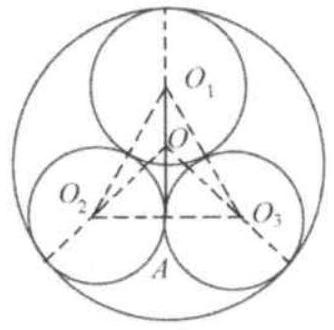
\includegraphics[width=\textwidth]{images/180(1).jpg}

Applying Pythagorean Theorem to Rt \(\triangle \mathrm{OO}_{2} \mathrm{~A}\) :\\
\(O_{2} A^{2}=O A^{2}+O_{2} A^{2} \Rightarrow \quad(r-5)^{2}=(12+8-r)^{2}+5^{2}\)\\
\(\Rightarrow \quad r=\frac{40}{3}=13 \frac{1}{3}\).\\

\end{document}
